Tensegrities share many of the design, fabrication, modeling, sensing,
and control challenges of the broader category of soft robots
\cite{Pfeifer:2012aa, Kim:2013aa, Majidi:2014aa},
which are made out of intrinsically soft and/or extensible
materials. 

\subsection{Opportunities in Morphological Computation}

%~\cite{2917079}

Both tensegrity and soft robots closely relate to the notion of
embodied intelligence, where morphology and materials can take over
some of the functions normally attributed to control to achieve a
system that is overall simpler, more robust and adaptive than those
based on the classical control paradigm. This principle
is known as \emph{morphological computation}~\cite{Pfeifer:2012aa,
Hauser}.  Many approaches to morphological
computation \cite{Zambrano:2014aa, Hauser} seek to reduce the
complexity of control systems through intelligent mechanism designs,
which effectively exhibit complex behaviors while reducing the use of
explicit control systems.  An example would be a compliant, soft hand
that naturally grasps a wide range of object shapes while executing
the same simple control law in all cases~\cite{Deimel:2015aa}.  These
systems may reduce the amount of sensing, actuation, or explicit
modeling and decision making associated with traditional approaches to
the task.

Tensegrity robots show this quality when they passively conform to the
environment and re-balance forces throughout their
structure \cite{Khazanov:2014aa}.  This is a very desirable property,
which enables the design of robots capable of a wide range of tasks
and activities. Such platforms are generally more versatile and robust
in the face of noise and the unpredictability of operating in messy
real-world environments.

%A well designed morphology can lead to drastic reductions in control
%requirements, as well as improved controllability. On the other hand,
%a poorly designed morphology may lead to low controllability, require
%complex control algorithms, or in the worse case, simply be inadequate
%for the task.

\begin{figure*}[t]
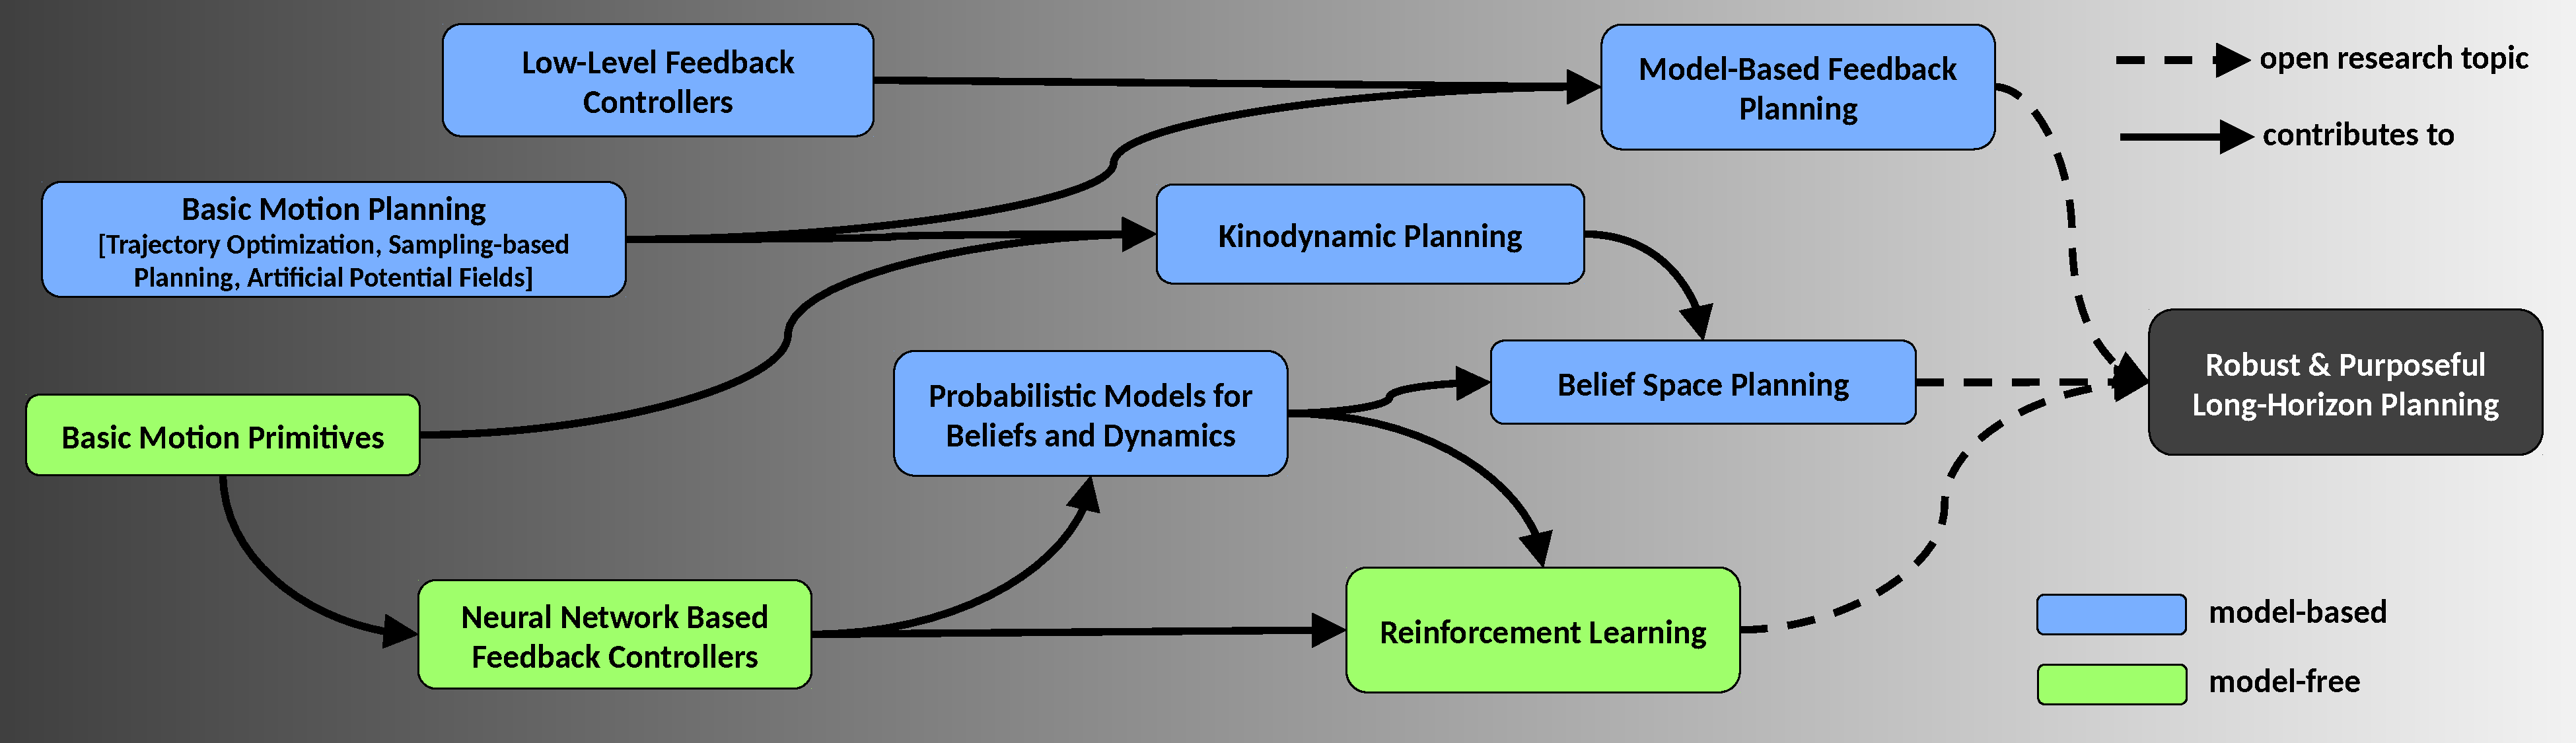
\includegraphics[width = \textwidth]{tex/img/review_overview_fig}
%\vspace{-.2in}
\caption{Overview of research topics discussed. An arrow indicates a topic that can contribute to the
development of another.  }
%\vspace{-.2in}
\label{fig:overview}
\end{figure*}

\subsection{Methods for Controlling Soft Robots}

Soft materials can bend, twist, stretch, compress, buckle, wrinkle and
so on. Such motions may involve an infinite number of DoFs indicating
that the control if soft robots requires new approaches
\cite{Rus:2015aa, Trimmer:2014aa}. While some progress can 
be made with more traditional control approaches, such as Model
Predictive Control ({\tt MPC}), these efforts typically require
accurate models of the robot and environment, which can be difficult
to acquire given the complex physical properties of soft robots.
Thus, many efforts focus specifically on biomimetic
systems \cite{Kim:2013aa}, which aim to reproduce the control
behaviors of their biological counterparts and often provide a new
understanding of soft organisms~\cite{Lin:2011aa}.

%This is similar to developments in tensegrity
%structures \cite{skelton_tensegrity_2009}.

To better understand the challenges in controlling soft and tensegrity
based robots, new static, kinematic and dynamic models have been
developed to capture the ability of bending and flexing
\cite{Saunders:2011aa, skelton_tensegrity_2009}.  For many
years, a popular abstraction for soft robots has been that of
piece-wise constant curvature ({\tt PCC})
\cite{Webster:2010aa}, which does not
capture all aspects of real mechanisms. Recently some non-constant
curvature models have been proposed to better model soft mechanisms.
\cite{Renda:2014aa}.  The need for
expressive models has also led to the development of simulation tools
targeted to soft robots \cite{Germann:2013aa}. This is also an
important development in tensegrity
robotics \cite{Caluwaerts2013rsif}, in which open source physics based
simulation tools have recently become
available \cite{SunSpiralSoftware}.  Table~\ref{tbl:resources} gives
pointers to simulation tools and analytical models for tensegrity
structures.

There have been both model-based and model-free approaches for the
low-level control of soft robots \cite{Rigatos:2009aa}. On the
model-based side, a recent effort utilizes finite
elements \cite{Largilliere:2015aa}, while a recent data-driven,
model-free approaches utilizes graph-theory \cite{Vikas:2015aa}.
There is no consensus, however, yet regarding the appropriate
methodology for control, and especially planning, for soft robots
given their highly continuous, complex and intrinsically compliant
deformation \cite{Rus:2015aa}.  This has motivated efforts in
proposing behavior-based control architectures for soft robots that
may be applicable to tensegrities as well \cite{Armbrust:2015aa}.  A
critical challenge in achieving deliberative control and planning,
shared between tensegrity structures and soft robots, is the
difficulty of solving the inverse kinematics problem. There are
solutions in certain setups, such as for semi-soft
manipulators \cite{Neppalli:2009aa}.

% or under the {\tt PCC} assumption \cite{Marchese:2014aa}.

\subsection{Planning for Tensegrities}

Similar to soft robots, the very properties that make tensegrities
ideal for physical interaction with the environment, such as
compliance, and multi-path load distribution, present some significant
challenges to traditional planning approaches and lead to uncertainty
during motion execution.

For instance, compliance allows tensegrity robots to adapt their shape
to workspaces of unknown or uncertain geometry. But when a force is
applied, the robot can deform in a non-linear manner and will often
excite oscillatory behaviors \cite{SunSpiral2013Tensegrity-Base}.  The
results of contacts are therefore very hard to predict to the level of
accuracy required for traditional trajectory and route planning
techniques.  These issues have limited investigation of planning
algorithms and focused most existing efforts on controllers for the
generation of local gaits \cite{Paul2006a} and quasi-static
paths \cite{Porta:2015aa}. Yet, they have also inspired the
development of approaches that go beyond the traditional control
toolkit and allow adaptation to multiple different terrain
types~\cite{MirletzSoftRobotics,burms2015online}.  Similar
developments in soft robotics technologies are taking place, which
address the complications of self-loading and non-linear compliance
\cite{Rus:2015aa}.  Recently, planning methods have been introduced 
which begin to address these needs for soft
robots \cite{Bonilla:2015aa, Marchese:2016aa}.

To move this field forward for both tensegrity and soft robots, both
high-level approaches of model-based and model-free planning should be
investigated as highlighted in Fig.~\ref{fig:overview}.  Model-based
planning approaches should be able to reason over more complex
dynamical models of tensegrity systems and provide robust trajectories
over probabilistic state representations that capture the diversity of
possible executions given the inherent uncertainty. Another direction
is to study feedback-based motion planners that provide a robust
composition of controllers with performance guarantees. In the
model-free domain, methods should capture the dynamics of low-level
controllers and then plan over the resulting dynamics. The low-level
controllers should manage the details of environmental interaction
while successfully driving the system to the next waypoint.

%The rest of this paper will aim to review work in low-level control
%and planning for tensegrity robots and outline directions for further
%research in this domain given developments in the motion planning and
%robot learning fields.

%Many advances have been made in understanding how to control robots
%with these physical properties, but those very same desirable
%properties introduce significant challenges to long-range planning
%algorithms.  Specifically, the adaptability of the robots and their
%ability to behave in complex ways which are outside the scope of the
%control system makes long range planning difficult because there is
%much greater uncertainty about the evolution of the robot's state as
%it executes the desired plan.

\begin{table}[b]
%\vspace{-.2in}
\centering
\begin{tabular}{r|r}
\textbf{resource} & \textbf{references} \\ \hline
\rowcolor[HTML]{BBDAFF} dynamics models   	& \cite{skelton_tensegrity_2009,hernandez2009reconfigurable,MiratsTur2009,sultan2002,Wroldsen2006A-Discussion-on}\\
kinematics \& statics
& \cite{C.R.1978,6907473,skelton_tensegrity_2009, 2003Tensegrity:-Str,Guest2010,Juan2008,pellegrino2014deployable}           \\
\rowcolor[HTML]{BBDAFF} simulation        	& \cite{SunSpiralSoftware,MirletzSoftRobotics,skelton_tensegrity_2009,Caluwaerts2013rsif,Rovira2009Control-and-Sim} \\
hardware design
                        & \cite{Bliss2013Central-Pattern,bohm2013vibration,Fest2004,Shibata2009,Caluwaerts2013rsif,miratstur2011athree-dof,kimrobust,Khazanov:2014aa,ChanMarch2004} \\
                        & \cite{Koizumi2012b,Paul2006a,Rieffel2009,Mirletz2015,sabelhaus2015system,bruce2014design,veuve2015deployment} \\
\rowcolor[HTML]{BBDAFF} state estimation        & \cite{Caluwaerts:2015aa} 
\end{tabular}
\caption{\vspace{-.05in}Resources for tensegrity control.}
%\vspace{-.4in}
\label{tbl:resources}
\end{table}

%dos2015design,fest2003adjustable
